% \chapter{Apache Kafka in caso d’uso simulato}
\chapter{Il percorso di stage}

\section{Formazione}

Il processo di Formazione ha avuto un importante ruolo all'interno dello \textit{stage}, con una durata complessiva di circa quattro settimane.
La causa di questo lungo periodo di formazione è data dallo studio di diversi ambiti e concetti per me nuovi, in particolare il settore del \textit{\acrlong{eai}} e la tecnologia di Kafka.

% \bigskip
\begin{figure}[h]
  \begin{center}
    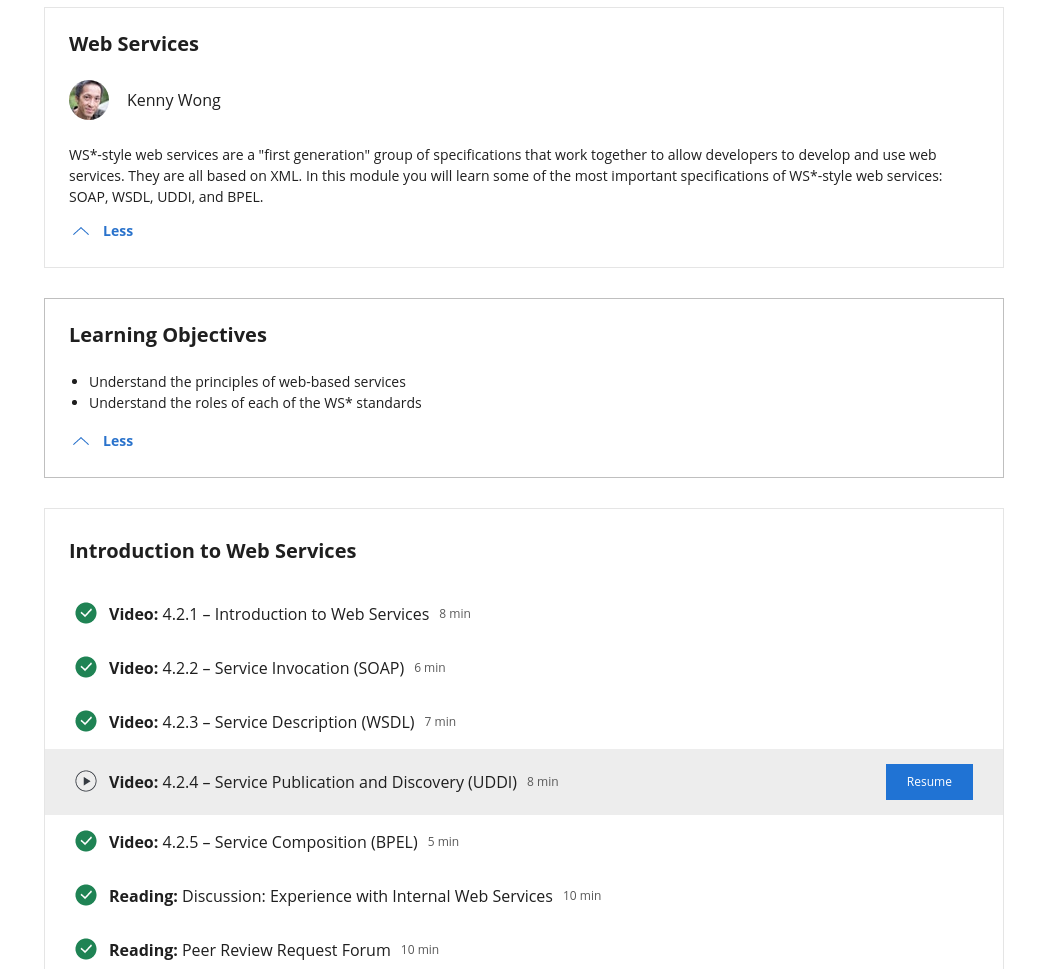
\includegraphics[width=0.7\textwidth]{images/coursera_week2.png}
    \caption{Screenshot del corso online \textit{acrlong{soa}} sulla piattaforma Coursera}
    \captionsetup{aboveskip=2pt}
    \caption*{\begin{footnotesize}\textit{Fonte: elaborazione personale}\end{footnotesize}}
  \end{center}
\end{figure}


Durante questo processo Sync Lab mi ha fornito del materiale didattico per l'apprendimento, quali diapositive e appunti di origine aziendale e l'accesso a dei corsi riguardo \textit{Software architecture}, \textit{\acrlong{soa}} (figura \thefigure) (tramite i corsi online su \textit{Coursera}) e Apache Kafka (tramite i corsi online su \textit{Udemy}).

Il tutor aziendale e responsabile \sacr{eai} hanno fornito durante i \textit{meeting} settimanali ulteriori chiarimenti e approfondimenti sul come Sync Lab applica questi concetti nello sviluppo di architetture \software.

Per i corsi online a maggiore contenuto nozionistico ho redatto degli appunti riassuntivi, con lo scopo di consolidare l'apprendimento e velocizzare la verifica del tutor aziendale.

\section{Analisi e modellazione di un caso d'uso}

Ad alcune videoconferenze ha partecipato anche un esperto \textit{senior} aziendale, esterno al progetto di \stage\ in questione, per illustrarmi un caso d'uso in cui l'azienda ha esposto un prototipo di sistema di integrazione utilizzando i concetti di \textit{Web Service}, \sacrfoot{soap} e \textit{request/response}, permettendomi la visualizzazione dei file \sacrfoot{wsdl}, \sacrfoot{xml} e \sacrfoot{xsd} associati.
Ho pertanto generato un caso d'uso adatto agli scopi dello \stage\ ispirandomi al caso d'uso reale illustrato.

Il caso d'uso modellato tratta una richiesta di credito telefonico da parte di un cliente ad un'azienda di telecomunicazioni tramite \textit{Web Service}, per soddisfare il requisito dello sviluppo della re-ingegnerizzazione del flusso di dati asincrono.
La \textit{request} avviene tramite flusso di un file \sacrfoot{json} che viene trasmesso attraverso i vari servizi che compongono il sistema di integrazione, basato sul \textit{Design Pattern} di tipo \textit{publish/subscribe}.

Va precisato che il contenuto di tale \sacr{json} non è strettamente rilevante allo sviluppo e funzionamento del \textit{Middleware}, ma aiuta a stabilire il contesto di utilizzo.

% \bigskip
% \begin{figure}[h]
%   \begin{center}
%     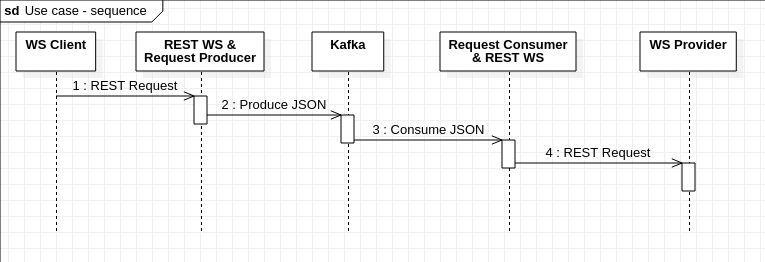
\includegraphics[width=\textwidth, trim={0.08cm 0 0 0.08cm},clip]{images/uc_sequence.png}
%     \caption{Diagramma di sequenza \sacr{uml} per il prototipo di caso d'uso iniziale}
%     \captionsetup{aboveskip=2pt}
%     \caption*{\begin{footnotesize}\textit{Fonte: elaborazione personale}\end{footnotesize}}
%   \end{center}
% \end{figure}

\noindent
Il caso d'uso è composto dai seguenti passaggi:
\begin{enumerate}
  \item il cliente (\textit{\sacrfoot{ws} Client}) effettua una richiesta di credito tramite invio di un file \sacr{json} al successivo Servizio Web in ascolto.
  \item il servizio composto da \sacrfoot{rest} \sacr{ws} e \textit{Request Producer} riceve il \sacr{json} e lo inserisce in Kafka tramite l'apposito \textit{Kafka Producer}, assumendo la funzione di \textit{publisher}.
  \item il servizio di \textit{Request Consumer}, sottoscritto al \textit{topic} in questione riceve il \sacr{json} e lo invia al \sacr{ws} finale tramite una \sacr{rest} request.
  \item il servizio in coda chiamato \sacr{ws} \textit{Provider} riceve il \sacr{json}; grazie ai dati ricevuti è in grado di fornire il servizio richiesto dal \textit{Client} nello \textit{step} 1.
\end{enumerate}

La modellazione dell'architettura e struttura del sistema da sviluppare seguirà questo prototipo di \sacrfoot{uc}.
Il modello associato al caso asincrono con \textit{callback} seguirà la stessa struttura e \textit{step} dello \sacr{uc} illustrato qui sopra, con l'aggiunta speculare del messaggio di ritorno.

\section{Progettazione architetturale}\label{sec:progettazione}
\subsection{Un \textit{middleware} basato su un \sacr{eda}}

La progettazione architetturale ha portato alla produzione di diversi diagrammi \sacr{uml} per rappresentare efficacemente l'architettura del prodotto e fornire un modello da seguire durante il processo di codifica.
Il processo ha richiesto frequenti \textit{meeting} e confronti per raggiungere un risultato finale soddisfacente al fine della sperimentazione.

La progettazione architetturale del prodotto comprende un \middleware\ centrale basato su di una \textit{\acrlong{eda}} con l'utilizzo di Apache Kafka, e due componenti di \textit{testing} chiamati \textit{service client} e \textit{service provider}, che simulano due servizi esterni che comunicano con il middleware attraverso \sacr{rest} \textit{request}.

Il sistema è composto da molteplici microservizi, che comunicano attraverso la rete di Docker.
L'obiettivo della progettazione è modellare un \middleware\ che sia implementabile in una \textit{\acrlong{soa}}, e consentirne la verifica e collaudo grazie ai servizi di \textit{testing}.

\begin{figure}[H]
  \begin{center}
    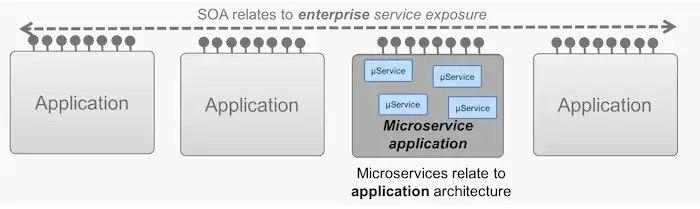
\includegraphics[width=0.7\textwidth]{images/soa_vs_micro.jpg}
    \caption{Visione ad alto livello delle differenze tra \sacr{soa} e microservizi}
    \captionsetup{aboveskip=2pt}
    \caption*{\begin{footnotesize}\textit{https://www.ibm.com/cloud/blog/soa-vs-microservices}\end{footnotesize}}
  \end{center}
\end{figure}

In figura \thefigure\ è rappresentata una visione ad alto livello dell'implementazione di un'applicazione a microservizi all'interno di una \sacr{soa}, evidenziando la differenza tra i due concetti.
% \bigskip

Per rappresentare in modo chiaro ed elegante il modello descritto dal \sacr{uc} sopra, ho elaborato diversi diagrammi \sacr{uml}.
% I diagrammi di maggiore rilevanza, oltre ad essere esposti all'interno di questa sezione accanto alla spiegazione associata, sono allegati in formato più grande a
Questi diagrammi rappresentano i componenti \textit{color coded}, notazione utilizzata per dare continuità e chiarezza attraverso le diverse tipologie di \sacr{uml} \textit{diagrams}.

\subsection{\sacr{uml} \textit{sequence diagrams}}

% \begin{figure}[H]
%   \begin{center}
%     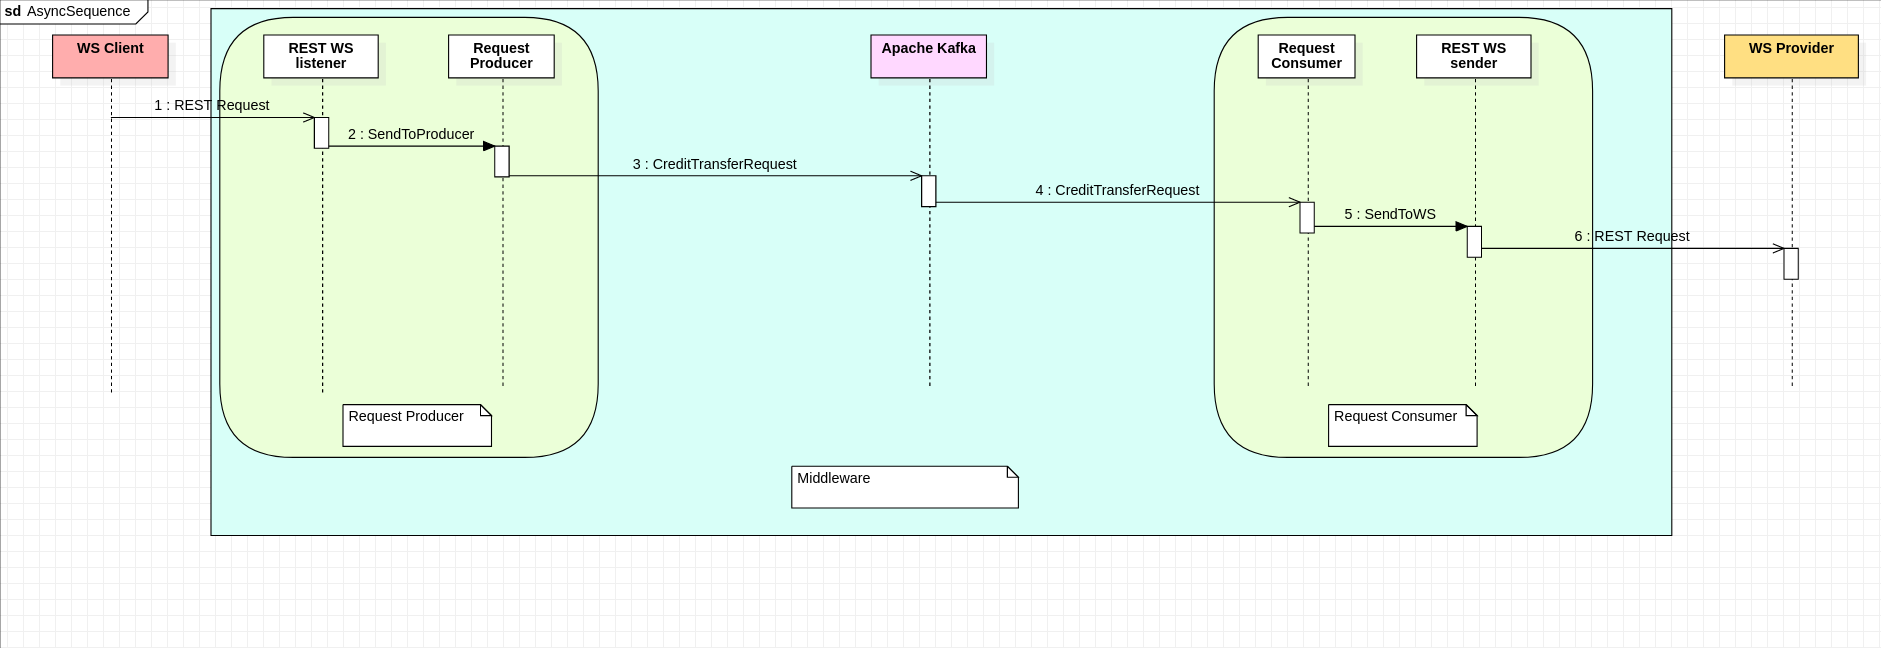
\includegraphics[width=\textwidth, trim={0.2cm 0 0 0.2cm},clip]{images/a_sequence2.png}
%     \caption{Diagramma \sacr{uml} di sequenza per la reingegnerizzazione del flusso asincrono}
%     \captionsetup{aboveskip=2pt}
%     \caption*{\begin{footnotesize}\textit{Fonte: elaborazione personale}\end{footnotesize}}
%   \end{center}
% \end{figure}

A partire dallo \sacr{uc} descritto nella sezione precedente, ho prodotto un \sacr{uml} \textit{sequence diagram} più approfondito per rappresentare il flusso del \sacr{json} tra i vari componenti.
% (figura \thefigure).

% \begin{figure}[h]
%   \begin{center}
%     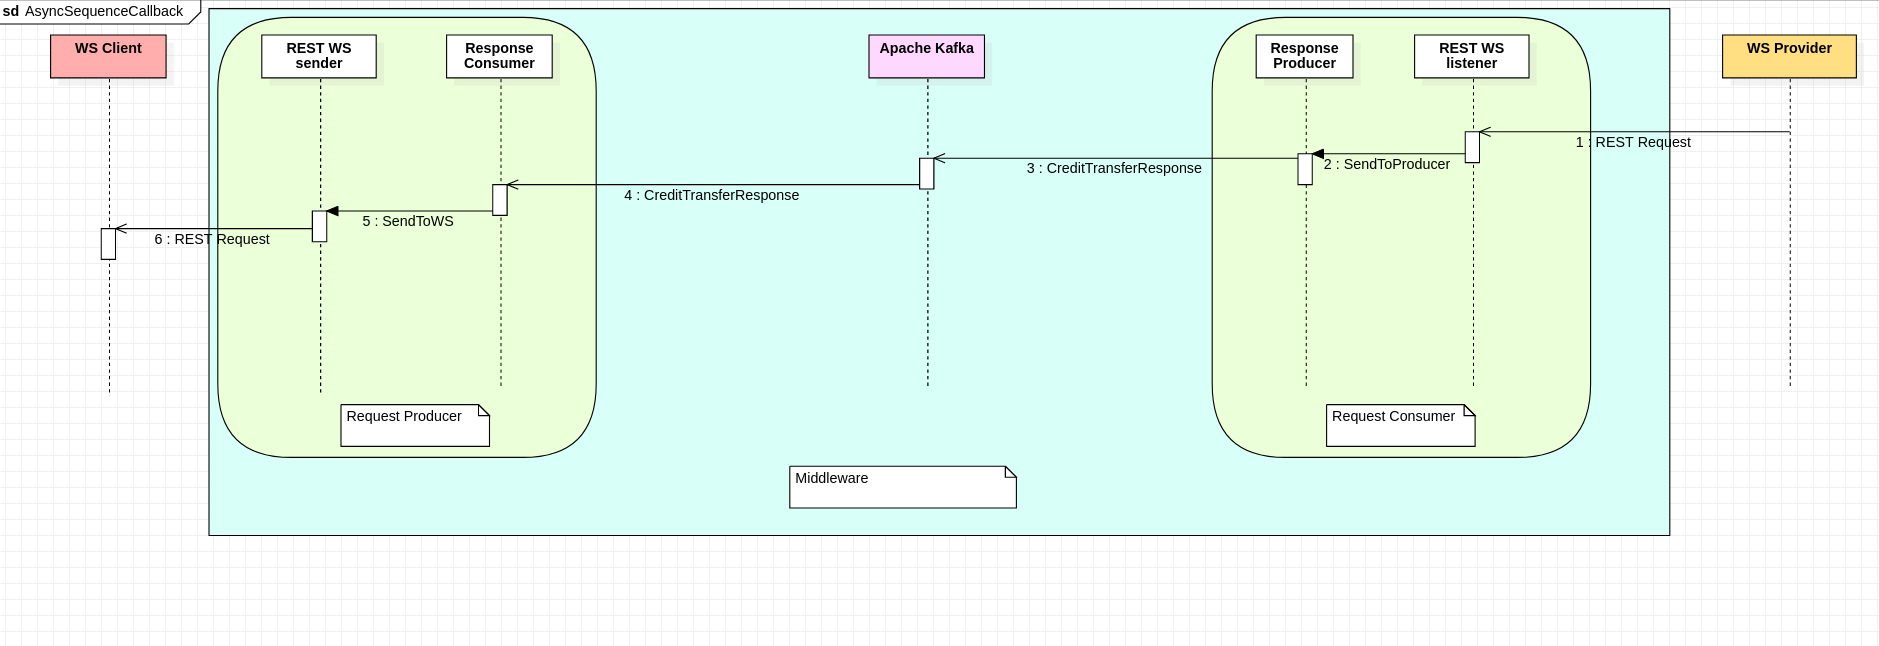
\includegraphics[width=\textwidth]{images/ac_sequence.png}
%     \caption{Diagramma di sequenza \sacr{uml} per la reingegnerizzazione del flusso asincrono con \textit{callback}}
%     \captionsetup{aboveskip=2pt}
%     \caption*{\begin{footnotesize}\textit{Fonte: elaborazione personale}\end{footnotesize}}
%   \end{center}
% \end{figure}

La progettazione del sistema associato al caso asincrono con \textit{callback} comprende lo stesso schema \sacr{uml} del caso asincrono, con aggiunta del flusso di ritorno speculare flusso di andata
% descritto nella figura \thefigure.

La re-ingegnerizzazione del flusso sincrono è stata scartata in favore dello studio di funzionalità aggiuntive tramite l'utilizzo della piattaforma di \textit{event streaming}.
La progettazione di un sistema basato su questo flusso era inizialmente prevista (come requisito desiderabile) nel piano di lavoro iniziale poiché associata ad un caso d'uso reale (di cui si è parlato nelle sezioni precedenti), ma infine è stata giudicata poco opportuna e fuori dagli scopi di Apache Kafka, un sistema basato sull'asincronismo.

Il tempo associato a tale requisito è stato pertanto riproposto per testare un'altra funzione utile in un \middleware\, quali la trasformazione di alcuni dati presenti nel \sacr{json}.
Più precisamente, è stato aggiunto un dato sensibile che viene nascosto e sostituito con asterischi "*" dopo la produzione del \textit{topic} in Kafka grazie all'utilizzo di Kafka Streams.
% \bigskip
\begin{figure}[h]
  \begin{center}
    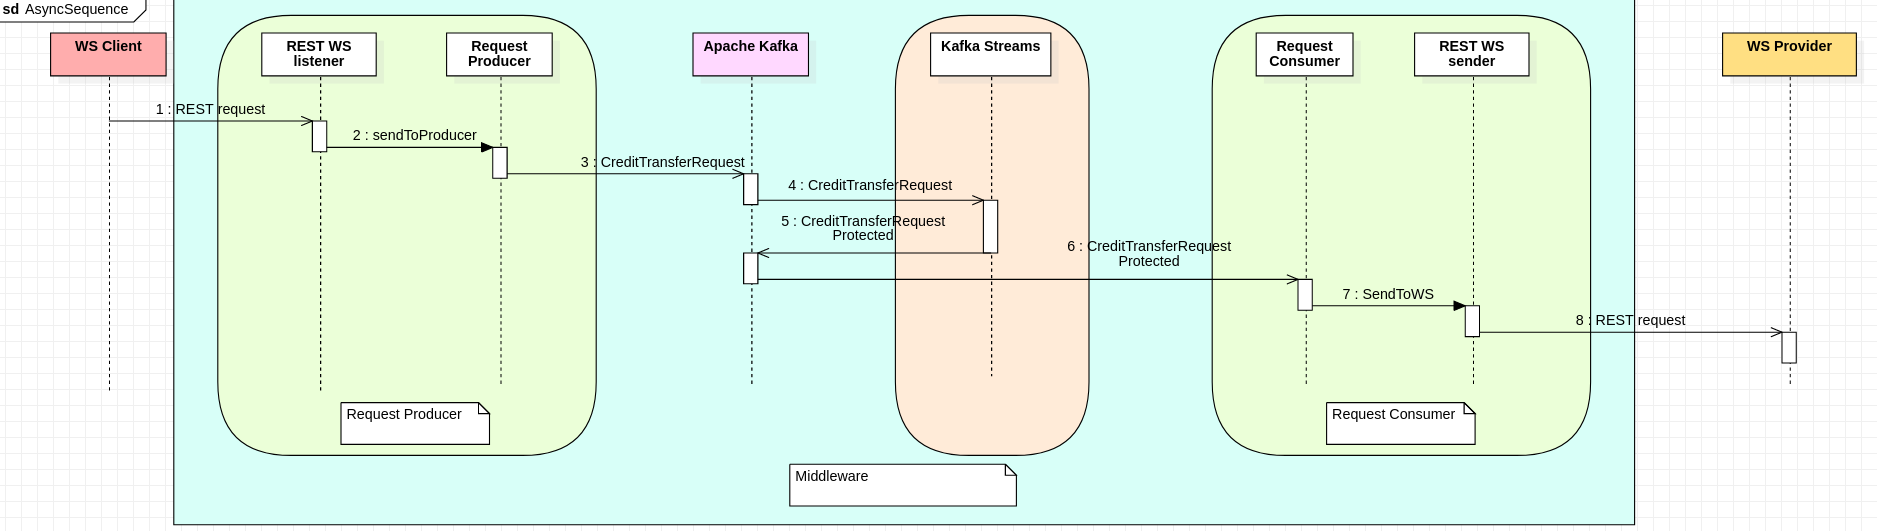
\includegraphics[width=\textwidth]{images/ap_sequence.png}
    \caption{Diagramma di sequenza \sacr{uml} per la re-ingegnerizzazione del flusso asincrono con protezione dei dati sensibili.}
    \captionsetup{aboveskip=2pt}
    \caption*{\begin{footnotesize}\textit{Fonte: elaborazione personale}\end{footnotesize}}
  \end{center}
\end{figure}

In figura \thefigure\ possiamo vedere il nuovo flusso asincrono con protezione (mascheramento) del dato sensibile.
La versione con \textit{callback} del flusso qui sopra prevede anche il flusso di ritorno (\textit{callback}), non illustrato in figura ma facilmente intuibile grazie al grafico che la precede.

\subsection{\sacr{uml} \textit{deployment diagram}}
\label{sub:uml_deployment}

A supporto di questi \sacr{uml} \textit{sequence diagram} che rappresentano efficacemente il flusso di dati, punto focale dell'intero sistema di integrazione (asincrono con la protezione del dato sensibile), ho prodotto ulteriori diagrammi, tra i quali il \textit{deployment diagram}.

\begin{figure}[h]
  \begin{center}
    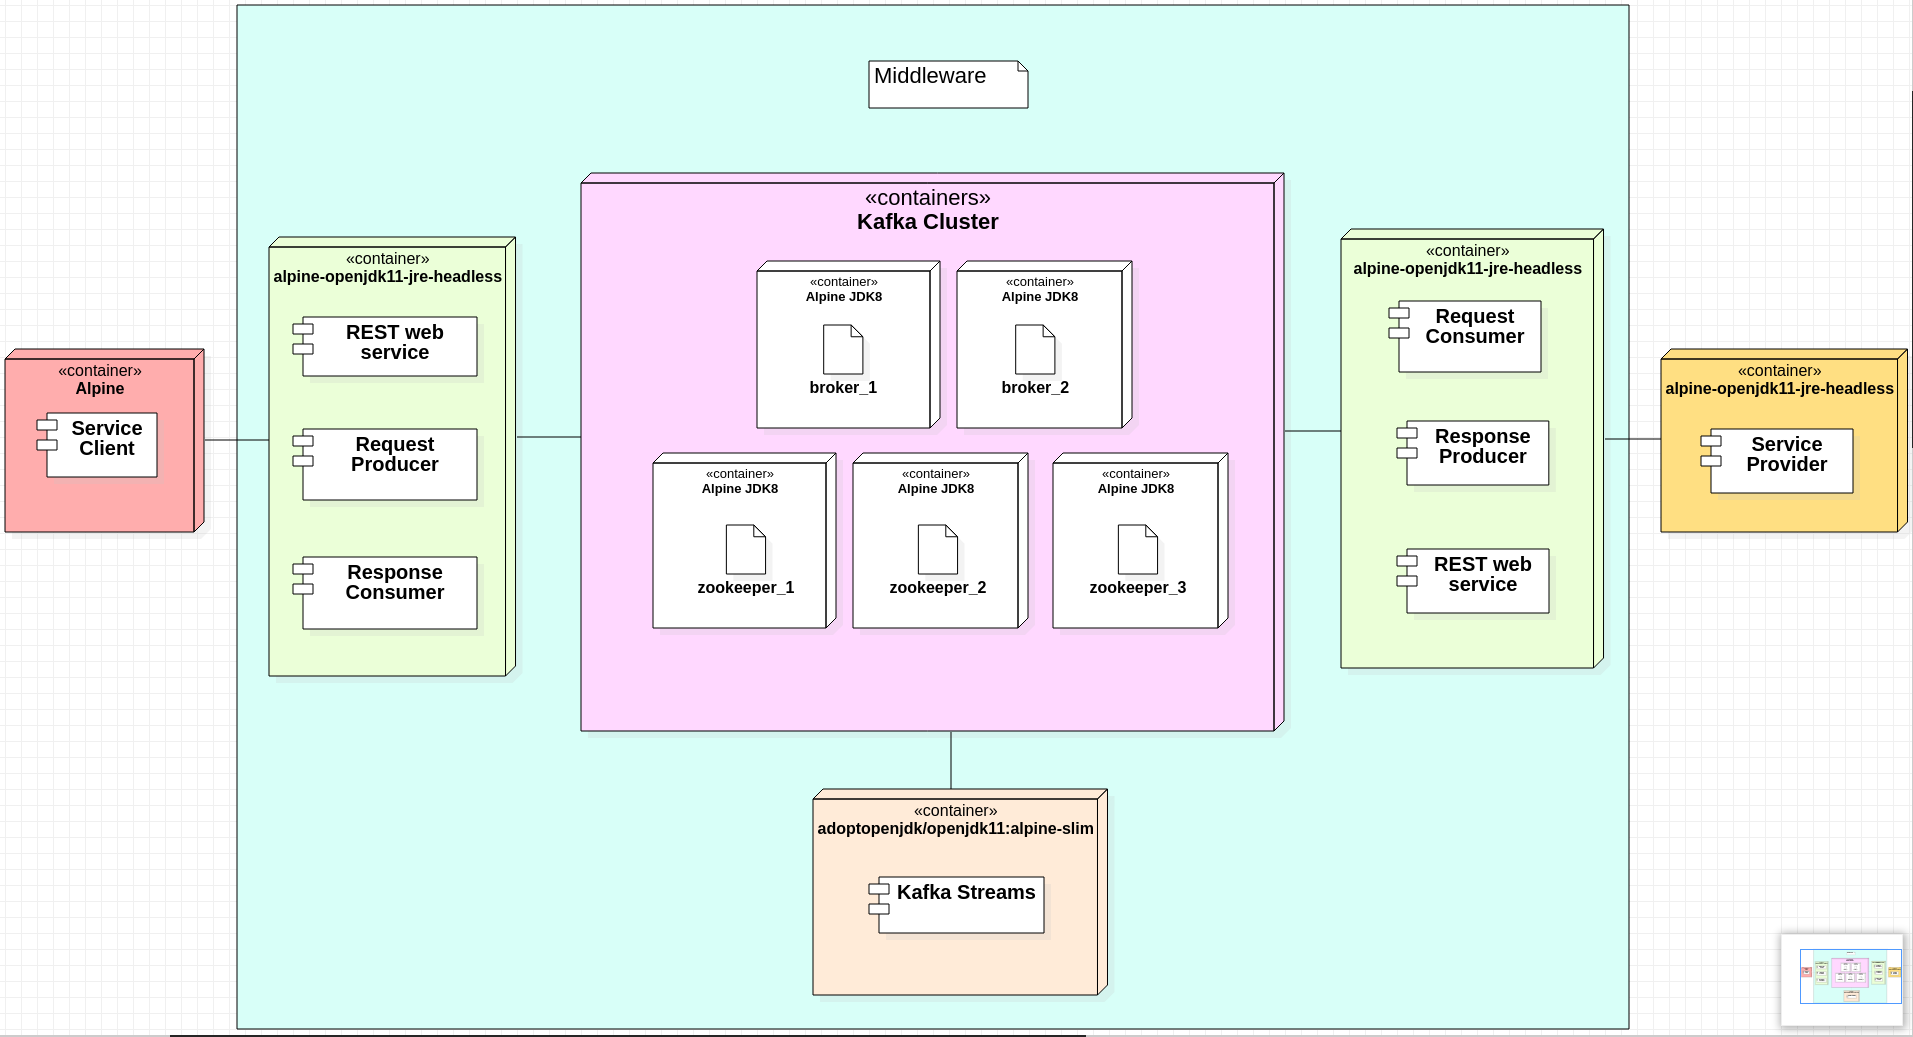
\includegraphics[width=\textwidth,  trim={0 0.2cm 0.2cm 0},clip]{images/ap_deployment.png}
    \caption{\sacr{uml} \textit{deployment diagram} per la re-ingegnerizzazione del flusso asincrono (protetto)}
    \captionsetup{aboveskip=2pt}
    \caption*{\begin{footnotesize}\textit{Fonte: elaborazione personale}\end{footnotesize}}
  \end{center}
\end{figure}

Questo diagramma (figura \thefigure) ha lo scopo di rappresentare la configurazione dei processi \textit{run time}, modellando la struttura di base in cui eseguono i diversi servizi;
il diagramma esprime l'ambiente in cui i vari componenti risiedono e ove essi comunicano tra di loro.

Con l'approvazione degli esperti aziendali, ho deciso di appoggiare il sistema di integrazione sulla piattaforma Docker.

Il diagramma di \textit{deployment} vede pertanto l'utilizzo di numerosi \textit{container} indipendenti che dialogano attraverso una rete locale all'interno di Docker.
Questi \textit{container} sono raffigurati dai vari nodi (rappresentati dai cubi in rilievo in figura).
A questa notazione fa eccezione il nodo virtuale intitolato "Kafka Cluster", che ha solamente lo scopo di raggruppare i vari nodi legati al \textit{environment} di Kafka con funzione comune, ma che in realtà non compone un container reale a se stante.
All'interno di questi nodi sono rappresentati gli artefatti che eseguono nel relativo \textit{container}, per esplicitare la presenza dei componenti.
Si può inoltre notare che l'ambiente di Apache Kafka è composto da un \textit{cluster} composto da due servizi \textit{Broker} e tre servizi \textit{Zookeeper}, allo scopo di simulare un caso d'uso reale in cui i diversi componenti sono distribuiti in sistemi indipendenti e garantiscono l'affidabilità dello \textit{streaming} di eventi.

\subsection{\sacr{uml} \textit{component diagram}}
\label{sub:uml_component}

\begin{figure}[H]
  \begin{center}
    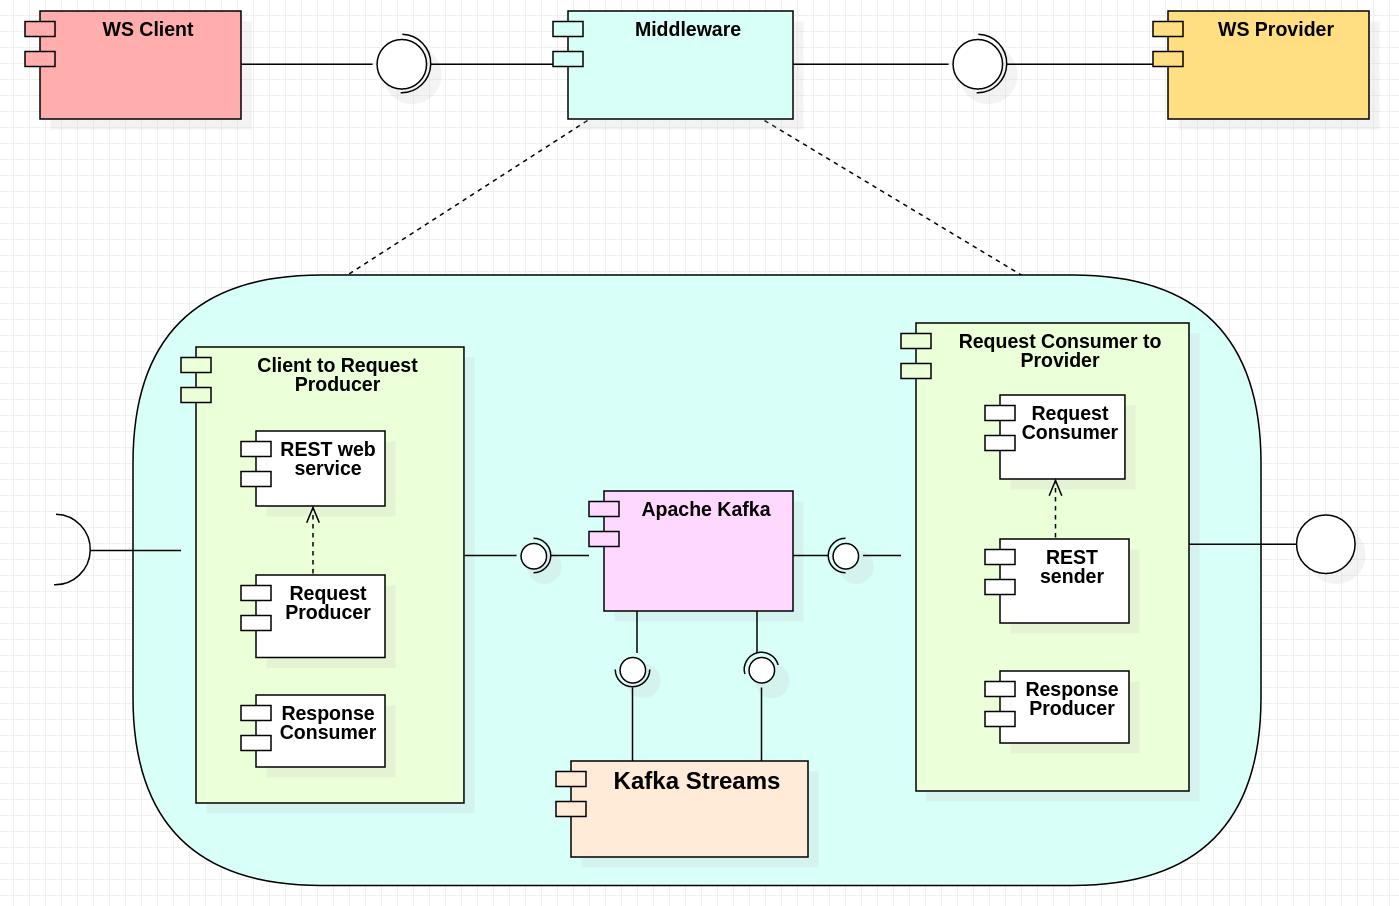
\includegraphics[width=\textwidth]{images/ap_component.png}
    \caption{\sacr{uml} \textit{component diagram} per la re-ingegnerizzazione del flusso asincrono (protetto)}
    \captionsetup{aboveskip=2pt}
    \caption*{\begin{footnotesize}\textit{Fonte: elaborazione personale}\end{footnotesize}}
  \end{center}
\end{figure}

Allo scopo di riassumere elegantemente i vari componenti del sistema ho elaborato un \sacr{uml} \textit{component diagram}.
Esso riassume con una visione ad alto livello i componenti che compongono il sistema e le modalità con cui esse interagiscono attraverso le relative interfacce.


% , basati su delle immagini Linux leggere e personalizzate.

% Come si può vedere dalla figura \thefigure,

% \section{\textit{Setup} dell'ambiente di lavoro}


\section{Codifica}

\subsection{Kafka \textit{cluster}}

Il primo passo del processo di codifica è stato quello del \textit{setup} dell'ambiente di Kafka in locale.
La guida rapida online fornita direttamente da Apache per un'installazione minimale di Kafka porta al \textit{download} di un pacchetto e l'esecuzione di un servizio Zookeeper e un \textit{broker} di Kafka.

Zookeeper è un servizio attualmente essenziale al funzionamento di Kafka, gestisce i nodi del \textit{cluster} e mantiene una lista dei \textit{topic} e dei messaggi.
Le versioni future di Kafka renderanno questo servizio non necessario, ma attualmente sono ancora in fase di sviluppo e non adatta all'ambiente di produzione.
I due \textit{broker} si occupano di ricevere i messaggi dai \textit{producer}.

Dopo un breve collaudo del corretto funzionamento dei servizi tramite l'inserimento di un evento in un \textit{topic} e la relativa lettura, ho iniziato ad espandere e trasportare il sistema su dei \textit{container} Docker.

Il \textit{cluster} di Kafka utilizzato nel progetto di \stage\ è composto dai componenti descritti dalla progettazione architetturale nella sezione precedente, ovvero tre servizi di Zookeeper e due \textit{broker} per rappresentare un sistema di piccole dimensioni che tuttavia si avvicina ad un caso d'uso reale poiché contiene multipli Zookeeper e multipli \textit{broker}.

Questi cinque servizi necessitano dunque di eseguire contemporaneamente in un ambiente "containerizzato" con Docker connessi alla stessa \textit{network} locale, che consente ai diversi servizi di scambiare messaggi tra di essi.

Ho implementato questo \textit{cluster} tramite un
\textit{file} di tipo \texttt{yml} utilizzato dall'estensione Docker-compose.

\noindent
Il \textit{file} contiene una lista di servizi, in cui in ognuno viene specificato:
\begin{itemize}
  \item l'immagine Docker su cui viene costruito il servizio o il \texttt{dockerfile} da utilizzare per la sua costruzione;
  \item il nome del \textit{container};
  \item il nome del servizio;
  \item le dipendenze funzionali del servizio;
  \item l'indirizzo \sacr{ipv4} statico e le porte attraverso cui è possibile raggiungere il servizio all'interno della rete locale dagli altri \textit{container}.
\end{itemize}

\subsection{\textit{Request producer} e \textit{request conconsumer}}

Il passo successivo è stato quello di sviluppare dei semplici \textit{producer} e \textit{consumer} in grado di inserire e leggere i dati in Kafka.
Una volta collaudati rapidamente questi due eseguibili scritti in Java, li ho incapsulati all'interno di un'applicazione utilizzando lo strumento di \textit{build} e gestione delle dipendenze Maven\footfullcite{maven}.

Per completare il modulo che costituisce il prototipo di \middleware\ è necessario che il \textit{producer} e \textit{consumer} siano in grado di comunicare con dei servizi esterni e fornire le interfacce adatte al ruolo.
Nel caso più complesso del flusso asincrono con \textit{callback}, entrambi questi servizi devono essere in grado di restare in ascolto di eventuali \sacr{rest} \textit{request} (che nel mio progetto utilizzano il protocollo \sacr{http}) e al tempo stesso di inviarle.

Ho pertanto creato un \sacr{http} \textit{server} minimale in Java attraverso il \textit{framework} Netty\footfullcite{netty}, in esecuzione in un \textit{thread} Java.
Sviluppi futuri vedrebbero probabilmente l'utilizzo di un \textit{framework} più evoluto come Spring Boot\footfullcite{spring}.
Un altro \textit{thread} si occupa invece dell'invio delle \sacr{rest} \textit{request} al servizio di destinazione, una volta ricevuto un evento da parte del relativo \textit{consumer}.
Per abbreviare, chiamerò il servizio che si interpone tra il \sacr{ws} \textit{Client} e Kafka "\textit{request producer}", e quello che si interpone tra Kafka e \sacr{ws} \textit{Provider} "\textit{request consumer}", in base al loro scopo principale: essi inviano e ricevono la \textit{request} relativa al dialogo dal \textit{client} al \textit{provider}.
% \bigskip
\noindent
L'insieme di questi componenti formano i blocchi logici illustrati in verde nella sezione precedente, in cui il servizio \textit{request producer} è formato da:
\begin{itemize}
  \item \sacr{rest} \textit{\acrlong{ws}} (\sacr{http} \textit{server} in ascolto della \textit{client request});
  \item \textit{client request producer};
  \item \textit{callback request consumer};
  \item \sacr{rest} \textit{\acrlong{ws}} (invio della \textit{callback request});
\end{itemize}
\noindent
e il \textit{request consumer} da:
\begin{itemize}
  \item \textit{client request consumer};
  \item \sacr{rest} \textit{\acrlong{ws}} (invio della \textit{client request});
  \item \sacr{rest} \textit{\acrlong{ws}} (\sacr{http} \textit{server} in ascolto della \textit{callback request});
  \item \textit{callback request producer}.
\end{itemize}

\subsection{\sacr{ws} \textit{Client} e \sacr{ws} \textit{Provider} }

Al fine di testare il prototipo di \middleware\ prodotto, ho realizzato due ulteriori \textit{container} con all'interno due eseguibili che si occupano di interagire con esso.

Il servizio intitolato \sacr{ws} \textit{Provider} è fondamentalmente simile ai servizi descritti nella sotto-sezione precedente: anch'esso possiede un \sacr{http} \textit{server} per rimanere in ascolto delle \sacr{rest} \textit{request} inviate dal \textit{request consumer} oltre ad un metodo per elaborare la \sacr{rest} \textit{request} di risposta associata al \textit{callback}.

L'altro servizio, che idealmente potrebbe essere molto simile al precedente servizio di test, in realtà presenta delle considerevoli differenze.
La causa di ciò non è una differenza reale in termini di funzionalità, quanto una questione di rapidità di \textit{testing} e codifica.

Il servizio è molto più leggero in termini di memoria, essendo composto da un semplice \textit{container} con una distribuzione di Alpine Linux\footfullcite{alpine}; esso possiede un'installazione del \software\ \texttt{curl} (accessibile via \sacr{cli}), ma è privo di ulteriori \software\ aggiuntivi da me prodotti.

Gli obiettivi di questo \sacr{ws} \textit{Client} sono legati a due \textit{network utility}: \texttt{curl} e \texttt{netcat}.
La prima mi permette di eseguire, interagendo manualmente con il \textit{container} tramite l'interfaccia \sacr{cli}, di eseguire \sacr{rest} \textit{request} con il \sacr{json} di partenza.
La seconda mi consente di restare in ascolto di eventuali \textit{request} su di una porta a mia scelta.

% I vantaggi di questa modalità manuale risiedono come anticipato nello sviluppo rapido, non solo di questo servizio ma anche dei restanti.
% Infatti grazie alle funzioni offerte da docker-compose, è semplice eseguire il \textit{restart} di un singolo \textit{container} contenente un servizio per testarne la nuova versione, e successivamente è sufficiente eseguire manualmente la \textit{request} dal \sacr{ws} \textit{Client} per verificare il funzionamento del sistema.

\subsection{Protezione dei dati sensibili con Kafka Streams}

Come visto nella sezione \ref{sec:progettazione}, alcuni dei dati trasmessi nel \sacr{json} vengono trasformati per mascherare i dati sensibili.

\noindent
Precisamente, il \sacr{json} passa dall'avere questa forma
% {\sacr{json} inviato al \middleware}
\begin{figure}[H]
  \begin{mycode}{json}
    {
      "CallerSystem": "Sistema chiamante 1",
      "PhoneNumber": "012345679",
      "Currency": "EUR",
      "Amount": "5",
      "Info": "Causale del Trasferimento Credito Residuo",
      "DebitType":"Bancomat",
      "CreditTransferDate": "2021-07-21",
      "CreditCardNumber": "1234567890123456"
    }
  \end{mycode}
  \caption{{\sacr{json} inviato al \middleware}}
  \captionsetup{aboveskip=2pt}
  \caption*{\begin{footnotesize}\textit{Fonte: elaborazione personale}\end{footnotesize}}

\end{figure}
\noindent
a questa
\begin{figure}[H]
  \begin{mycode}{json}
    {
      "CallerSystem": "Sistema chiamante 1",
      "PhoneNumber": "012345679",
      "Currency": "EUR",
      "Amount": "5",
      "Info": "Causale del Trasferimento Credito Residuo",
      "DebitType":"Bancomat",
      "CreditTransferDate": "2021-07-21",
      "CreditCardNumber": "****************"
    }
  \end{mycode}
  \caption{\sacr{json} protetto, ricevuto al termine del \textit{callback}}
  \captionsetup{aboveskip=2pt}
  \caption*{\begin{footnotesize}\textit{Fonte: elaborazione personale}\end{footnotesize}}
\end{figure}
\noindent
in cui si può notare che l'ultimo dato ha subito la modifica descritta.

Ho implementato questa funzione utilizzando Kafka Streams\footfullcite{streams}, che permette di leggere un \textit{topic} e modificarlo istantaneamente per un'elaborazione in \textit{real time}.

\subsection{Efficienza nello sviluppo}

Durante la codifica, ho adottato diverse misure per minimizzare il tempo necessario.
Questi provvedimenti riguardano principalmente l'ottimizzazione del sistema di \textit{container}, non allo scopo di migliorare l'efficienza, rapidità d'esecuzione e di \textit{build} del prodotto finale (che è stata comunque raggiunta come effetto secondario) ma a quello di ridurre il tempo e risorse necessarie per il \textit{testing}, riducendo di conseguenza le ore e le risorse necessarie allo sviluppo.

Tutti le misure prese sono strettamente legate alla mia famigliarità con alcune tecnologie e al risorse personali richieste per l'apprendimento e sviluppo di una nuova funzionalità.

\noindent
Elenco i principali provvedimenti intrapresi per minimizzare il tempo di sviluppo:
\begin{itemize}
  \item \textbf{ottimizzazione delle risorse utilizzati dai \textit{container}}.
  Molti dei container prodotti possiedono delle versioni \textit{premade} sulla libreria di DockerHub\footfullcite{dockerhub} (ad esempio i \textit{container} che formano il \textit{cluster} di Kafka).
  Tuttavia, utilizzare delle versioni \textit{ad-hoc} da me costruite mi ha permesso di ridurre considerevolmente le dimensioni del \textit{container} e mantenere solamente le funzioni a me necessarie, e conseguentemente ridurre il tempo della \textit{build} delle immagini e la loro esecuzione. Dato le numerose operazioni di \textit{build} e \textit{testing}, nel lungo termine ha portato ad un risparmio di tempo significativo.
  \item \textbf{invio della richiesta \sacr{rest} del \textit{service client} tramite \sacr{cli}}.
  I vantaggi di questa modalità manuale risiedono come anticipato nella rapidità di sviluppo, non solo di questo servizio ma anche dei restanti.
  Infatti grazie alle funzioni offerte da docker-compose, è semplice eseguire il \textit{restart} di un singolo \textit{container} contenente un servizio per testarne la nuova versione, e successivamente è sufficiente eseguire manualmente la \textit{request} dal \sacr{ws} \textit{Client} per verificare il funzionamento del sistema.
  È sicuramente possibile l'automatizzazione di questo processo (ad esempio effettuando richieste continue in modo automatico) ma l'implementazione di questa funzione avrebbe, secondo la mia stima personale, richiesto più tempo della soluzione attuata o posto problemi nel filtro dell'\textit{output}.
  \item \textbf{la \textit{build} delle applicazioni costruite con Maven avviene in locale}.
  Questo porta a due vantaggi.
  Il primo è che la \textit{build} impiega meno tempo, dato che non è necessario lanciare alcun \textit{container} e Maven non deve sincronizzare o controllare la versione delle dipendenze online più di volte (è possibile  disattivare la sincronizzazione, ma richiede comunque più tempo).
  La seconda, più importante, è che l'immagine Docker stessa non richiede né \textit{build} né Maven.
  Il \textit{container} si occupa solamente di copiare l'eseguibile pre-costruito al suo interno e di eseguirlo con Java.
\end{itemize}

\section{Prodotto finale, verifica e collaudo}

\subsection{Prodotto finale}


Il prodotto finale del progetto è composto da i diversi componenti illustrati nella sotto-sezione \ref{sub:uml_component}, per un totale di dieci servizi ognuno nel proprio
\textit{container} Docker (conformi con il \textit{deployment diagram} alla sotto-sezione \ref{sub:uml_deployment}).
Una visione ad alto livello può esprimere il prodotto risultante dallo \stage\ come \textbf{due servizi di test quali \sacr{ws} \textit{Client} e \sacr{ws} \textit{Provider} che scambiano messaggi sotto forma di \texttt{file} \sacr{json} tramite un \middleware\ basato su Apache Kafka in un'architettura focalizzata sugli eventi.}
Il\middleware\ presenta inoltre la funzionalità aggiuntiva di trasformazione dei dati grazie all'utilizzo di Kafka Streams.

Tra i diversi servizi prodotti, tre risultano più strutturati e complessi, ovvero il \textit{request producer}, \textit{request consumer} e il \sacr{ws} \textit{Provider}.
Questi infatti sono degli applicativi \textit{multi-thread}, con struttura generata da Maven e formati da diversi \texttt{file} Java che si occupano di inviare e ricevere \sacr{rest} \textit{request}, "produrre" e "consumare" i dati utilizzando Kafka.

\begin{figure}[H]
  \begin{center}
    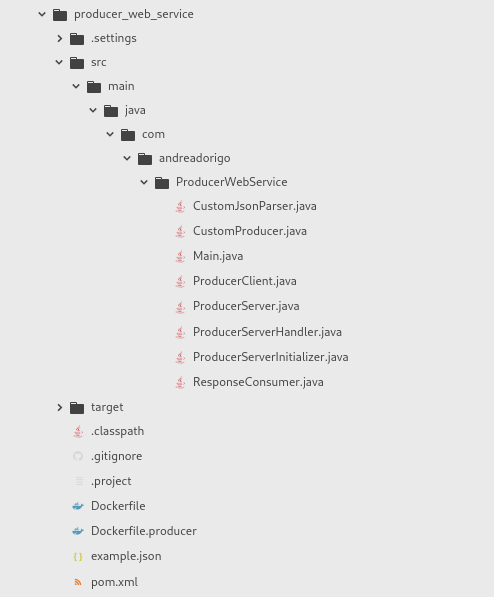
\includegraphics[width=0.5\textwidth]{images/folder_tree.png}
    \caption{\textit{Folder tree} dell'applicativo relativo al servizio \textit{request producer}}
    \caption*{\begin{footnotesize}\textit{Fonte: elaborazione personale}\end{footnotesize}}
  \end{center}
\end{figure}

I cinque servizi del \textit{cluster} di Apache Kafka risultano relativamente semplici: sono composti da un'immagine di Alpine Linux con un'installazione di Java \sacrfoot{jre} versione 8, con all'interno gli eseguibili di Kafka e i file di configurazione personalizzati per il \textit{setup} del cluster (porte e indirizzi).

Il servizio che compone il \sacr{ws} \textit{Client} è quello di dimensioni più ridotte, essendo composto da un'immagine minimale di Linux con all'interno le \textit{network utility} trattate in precedenza.

Infine, il servizio che utilizza Kafka Streams per il mascheramento dei dati sensibili è simile ai primi tre, con la differenza che esso non richiede dei processi \textit{multi-thread} ma solamente un'unica classe Java per il processo di \textit{streaming} dei messaggi.

Nella figura \ref{fig:riass_componenti} è presente una bozza riassuntiva dei componenti e della loro comunicazione, presa dalla \textit{board} di progetto ClickUp.

\begin{figure}[h]
  \begin{center}
    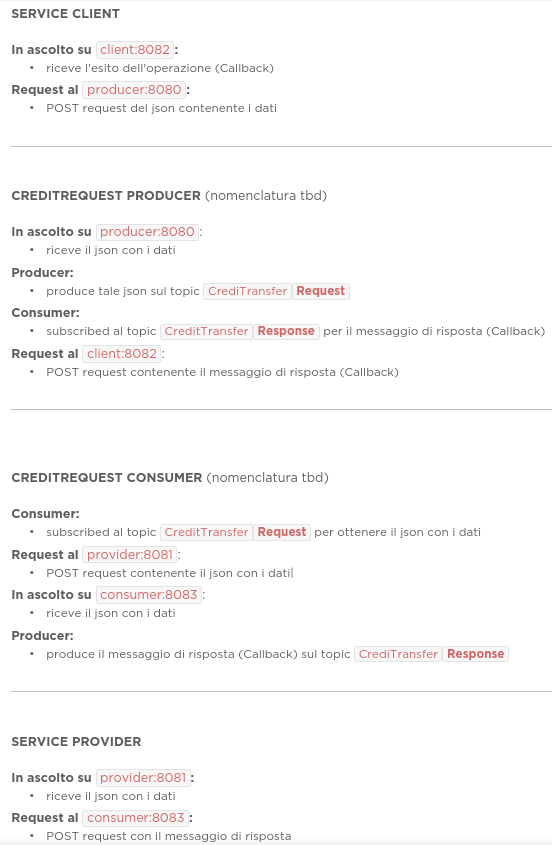
\includegraphics[width=0.60\textwidth]{images/riass_componenti.png}
    \caption{\sacr{uml} Riassunto dei componenti prodotti nel caso asincrono con \textit{callback} e della loro comunicazione}
    \captionsetup{aboveskip=2pt}
    \caption*{\begin{footnotesize}\textit{Fonte: elaborazione personale}\end{footnotesize}}
    \label{fig:riass_componenti}
  \end{center}
\end{figure}



L'immagine illustra i servizi prodotti per il flusso asincrono con \textit{callback} e di come essi comunichino tra di loro attraverso le varie porte, elaborata durante il processo di Progettazione iniziale (si può notare come non sia ancora presente la protezione del dato sensibile con Kafka Streams, funzionalità aggiunta negli ultimi giorni di \stage).


\subsection{Verifica}


% Questi microservizi hanno raggiunto efficacemente il risultato preposto, creando il sistema richiesto dalla sperimentazione; i due servizi di test quali \sacr{ws} \textit{Client} e \sacr{ws} \textit{Provider} si scambiano messaggi tramite un \middleware\ basato su Apache Kafka.
Il tempo dedicato al processo di Verifica è stato relativamente breve rispetto alla maggior parte dei prodotti \software: la causa di questa durata minore è la natura sperimentale del progetto di \stage\ che, come visto nella sotto-sezione \ref{sub:obiettivi_stage}, è incentrato sulla re-ingegnerizzazione del flusso di dati ma senza l'obiettivo di produrre un \middleware\ da implementare in produzione (quest'ultimo è un obiettivo aziendale nel lungo termine, ma non di questo specifico progetto di sperimentazione).
Il processo di Verifica è stato applicato per tutta la durata del processo di Codifica, con particolare attenzione nelle fasi finali.

Il prodotto è stato più volte verificato con la supervisione del tutor aziendale e il responsabile del \sacr{eai}.
Tutti i \textit{container} prodotti sono stati revisionati, compresa la loro corretta esecuzione.
I passaggi principali del processo hanno visto la verifica manuale dell'\textit{input} e \textit{output} di ogni singolo \textit{container} sia nel flusso di dati in andata che nel flusso di ritorno di \textit{callback}, con eccezione del \textit{cluster} Kafka.
La stampa su console del movimento del dato, contenuta nei servizi scritti in Java, ha aiutato la verifica costante della funzionalità principale permettendo il rilevamento immediato di casi di regressione.
Il \textit{cluster} Kafka invece è stato il soggetto di una verifica differente: ho analizzato approfonditamente l'output in console dei vari \textit{container}, per assicurarmi la corretta comunicazione tra di essi.
Tramite l'utilizzo degli eseguibili di supporto messi a disposizione dal \textit{team} di Apache Kafka, ho periodicamente controllato i contenuti dei \textit{topic} generati durante il progetto ed il corretto funzionamento del \textit{cluster}.


\subsection{Collaudo}

% Il tempo dedicato al processo di Collaudo è stato relativamente breve rispetto alla maggior parte dei prodotti \software: la causa di questa durata minore è la natura sperimentale del progetto di \stage\ che, come visto nella sotto-sezione \ref{sub:obiettivi_stage}, è incentrato sulla re-ingegnerizzazione del flusso di dati ma senza l'obiettivo di produrre un \middleware\ da implementare in produzione (quest'ultimo è un obiettivo aziendale nel lungo termine, ma non di questo specifico progetto di sperimentazione).
Come per il processo di Verifica, anche il processo di Collaudo ha visto un utilizzo di risorse ridotto rispetto a quelle richieste per un \software\ da distribuire in produzione.

Il processo è stato effettuato con la supervisione del tutor e degli esperti aziendali.
hanno visto il processo di \textit{build} e successivo avvio simultaneo di ogni singolo servizio all'interno del \textit{cluster} tramite l'apposito comando di Docker-compose "\texttt{docker-compose up --build}".

Dopodiché, al fine di testare che il \software\ eseguisse effettivamente le funzioni richieste dal progetto di sperimentazione (\textit{test} d'efficacia), ho effettuato delle \sacr{http} \sacr{rest} \textit{request} contenenti il \sacr{json} con i dati.
Ho eseguito questo collaudo tramite una connessione manuale al \textit{container} contenente il servizio \sacr{ws} \textit{client}, per poi dare manualmente il comando di \textit{request} grazie all'\textit{utility} \texttt{curl}.
L'analisi del \sacr{json} in entrata e in uscita dal sistema hanno garantito l'efficacia del \software\ sperimentale prodotto: la richiesta contenente i dati necessari viene correttamente trasmessa dal cliente al fornitore di tale servizio, e infine il cliente riceve un messaggio di risposta (\textit{callback}, in questo caso sperimentale la risposta è un semplice inoltro dei dati di partenza).

Per dimostrare i risultati raggiunti e le capacità del prodotto finale, esso è stato presentato all'azienda in conclusione del percorso di \stage\ in un \textit{online meeting}.
Il \textit{meeting} si è tenuto in due fasi distinte: la prima costituita da un'introduzione concettuale dell'architettura e degli scopi del percorso di \stage\ tramite l'aiuto di alcune diapositive da me prodotte, e la seconda da una dimostrazione \textit{live} del \software\ in esecuzione tramite la condivisione dello schermo.

% TODO: expand
% Come si può osservare
